\documentclass[12pt]{amsart}
\usepackage{geometry}
\geometry{letterpaper}
%\usepackage[parfill]{parskip}
\usepackage{graphicx}
\usepackage{amssymb}
\usepackage{epstopdf}
\usepackage{listings}
\DeclareGraphicsRule{.tif}{png}{.png}{`convert #1 `dirname #1`/`basename #1 .tif`.png}

\title{Midterm Report: The Billiard Problem}
\author{Phil Mayer}

\begin{document}
\maketitle

\section{Background}
For my midterm project, I decided to study the billiards problem. Overall, it interested me most because the behavior of a billiard ball can
demonstrate chaotic behavior; even with seemingly simple assumptions like mirror-like collisions, the billiard's motion is complex and depends
highly on the initial conditions. 

The problem begins by considering a billiard ball placed at some initial position $(x_0, y_0)$ on a table. We can consider tables of different sizes
and dimensions, for example rectangles, circles, and other ``stadium" configurations. We impart the billiard ball with some initial velocity 
$\vec{v}$, then follow its motion given by the following differential equations:
\[
	\frac{dx}{dt} = v_x \: , \qquad
	\frac{dy}{dt} = v_y
\]
\newline
While we can also account for energy loss due to friction and collisions with the table boundaries later on, we can assume that the kinetic
energy of the ball (and thus the magnitude of its velocity) remains constant. We also make the assumption that when the ball hits one of the
table boundaries, that the collision is perfectly elastic and mirror-like; in other words the billiard's angle of incidence $\theta_i$ with the wall is
equal to its angle of reflection $\theta_f$:
\[
	\theta_i = \theta_f
\]
\newline
Our task is then to plot the trajectory of the ball. While the trajectory is simple to plot between collisions (by Euler's method), some basic vector
manipulation is required to determine the new velocity vector after the collision. If we suppose the initial velocity before a given collision
can be denoted $\vec{v}_i = [ (v_i)_x, (v_i)_x ]$, then the components of the post-collision velocity vector $\vec{v}_f$ depend on which 
component of $\vec{v}_i$ was perpendicular and parallel to the table boundary. In short, given the perpendicular component $(v_i)_\perp$ and
the parallel component $(v_i)_\parallel$, we get the components of the reflected velocity vector as:
\[
	(v_f)_\perp = - (v_i)_\perp \: , \quad (v_f)_\parallel = (v_i)_\parallel
\]
While this is conceptually fairly straight-forward, the implementation is relatively difficult. A number of interesting difficulties arise, as I discuss in
the next sections.

\section{Numerical Methods}
To solve the billiards problem numerically, we use Euler's method to solve the following ODE's from last section:
\[
	\frac{dx}{dt} = v_x \: , \qquad
	\frac{dy}{dt} = v_y
\]
\newline
As we have seen many times in class, after providing some initial conditions, the motion of the ball at time step $i$ in $x$ and $y$ is given by:
\[
	x_i = x_{i-1} + \frac{dx}{dt} \Delta t = x_{i-1} + (v_x)_{i-1} \Delta t
\]
\[
	y_i = y_{i-1} + \frac{dy}{dt} \Delta t = y_{i-1} + (v_y)_{i-1} \Delta t
\]
\newline
We can derive these two results by recalling that in order to estimate $\frac{dx}{dt}$ and $\frac{dy}{dt}$, we can use backwards differencing as
follows for all indices $i \leq N$ for some number of points $N$:
\[
	\frac{dx}{dt} \approx \frac{x_i - x_{i - 1}}{\Delta t} \:, \quad \frac{dy}{dt} \approx \frac{y_i - y_{i - 1}}{\Delta t}
\]
\newline
We then rearrange the two equations to obtain:
\[
	x_i = x_{i-1} + \frac{dx}{dt} \Delta t \: , \quad y_i = y_{i-1} + \frac{dy}{dt} \Delta t
\]

To calculate the new velocity vector after a collision, no overly complex numerical methods are required.

\section{Results}
For my solution to the billiards problem, I decided to focus on having the most correct (bug-free) implementation, thus was only able to focus
on the case of a square table. I considered the table to be a square region from $x = -1$ to $x = 1$ and $y = -1$ to $y = 1$. I chose to place
the ball at the origin for the sake of simplicity, so $(x_0, y_0) = (0, 0)$ in all executions of my program. To allow the user to experiment with
some different parameters, I left the choice of number of points, time precision, initial velocity and initial angle all the user. Default values are
used if invalid parameters are selected, for example a negative number of points $N$.

The major problem I encountered while implementing my solution was accurate collision detection, particularly around the corners. After writing
my initial version of the program, I noticed that for large values of $N$ and large time steps $\Delta t$, the billiard ball would eventually escape
the corners of the table. The problem was largely caused by the following lines of code, which calculated the new velocity vector after
a collision was detected:
\newline
\begin{lstlisting}
if ((x[i] > xMax || x[i] < xMin) && (y[i] > yMax || y[i] < yMin)) {
	vx[i] = -vx[i-1];
	vy[i] = -vy[i-1];
}
else if (x[i] > xMax || x[i] < xMin) {
	vx[i] = -vx[i-1];
	vy[i] = vy[i-1];
}
else {
	vx[i] = vx[i-1];
	vy[i] = -vy[i-1];
}
\end{lstlisting}

While this algorithm does detect collisions in the corners of the table by simply changing the sign of both components of the velocity, it does
not handle corner collisions effectively enough. The main issue with this approach is that it does not account for the following situation: suppose
the billiard collides with the table boundaries in $x$ and is very close to colliding in $y$. This algorithm adjusts the $x$ component of the velocity
accordingly, but on the next time step, the billiard may be off the table in the $y$ direction. My solution solves this problem by detecting this exact
scenario.

Overall, my implementation runs fairly well, but does not demonstrate the chaotic behavior seen in the ``stadium" table configurations discussed
in the textbook. For example, consider the following trajectory and phase-space plots generated by my program for $N = 10000$ points, a time
step of $\Delta t = 0.01$, an initial velocity of $4.0$ m/s, and an initial angle of $\theta = 17^{\circ}$:

\begin{center}
	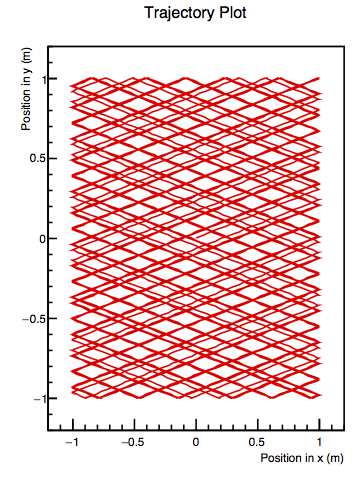
\includegraphics{graph1.png}
	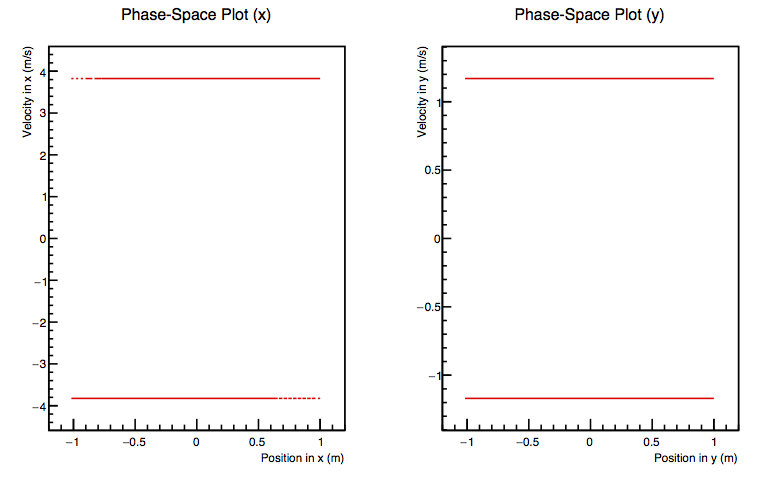
\includegraphics{graph2.png}
\end{center}

In future versions of my program, I would generalize the program to be able to handle different table geometries, like circular or ``stadium"
configurations in which chaos can be seen. It would also be interesting to allow the user to set the initial position of the billiard, which would be a
minor change.

\section{Stability of the Numerical Method}
Overall, the program's behavior is stable given reasonable choices for $\Delta t$, the time step size, and the initial velocity vector. Time steps
above $\Delta t = 2$ tend to be unreliable, given high velocities as well. Low-magnitude velocities and small time steps, however, help the
program behave predictably and accurately. Problems that arise during executions of the program are not typically caused by approximation
error in Euler's method; they tend to be caused by collisions around the corners. For example, given $N = 10000$, a time step size of
$\Delta t = 20$, an initial velocity of $v = 20$ m/s, and an angle of $\theta = 10^{\circ}$, we see that the billiard is able to escape out of both
corners in the following example:
\begin{center}
	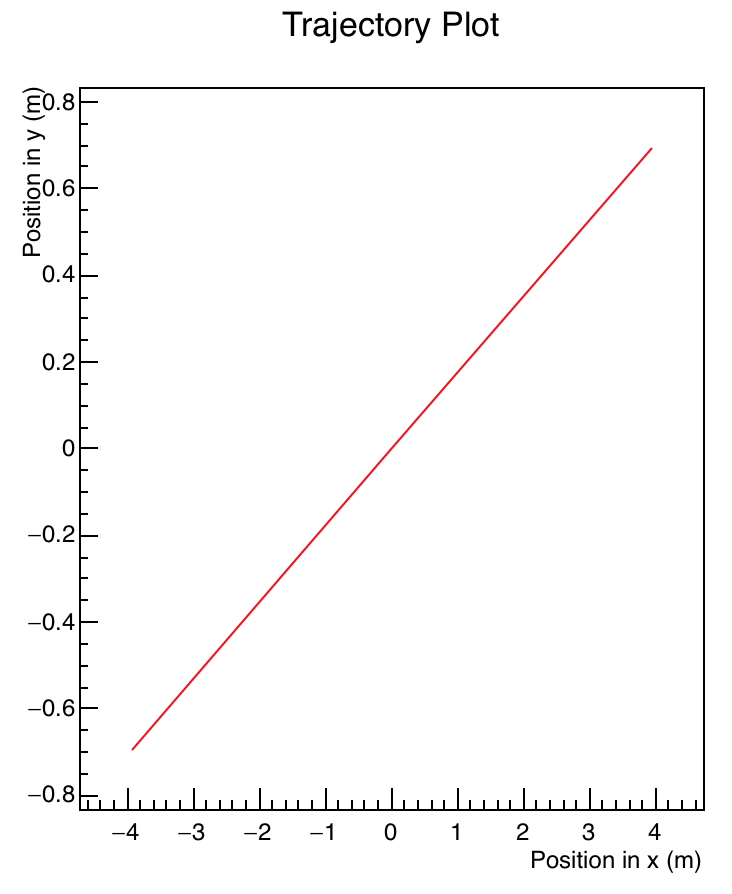
\includegraphics[scale=0.5]{graph3.png}
\end{center}


\end{document}  